% Created 2017-02-22 Wed 16:47
% Intended LaTeX compiler: pdflatex
\documentclass[10pt,aspectratio=1610]{beamer}
\usepackage[utf8]{inputenc}
\usepackage[T1]{fontenc}
\usepackage{graphicx}
\usepackage{grffile}
\usepackage{longtable}
\usepackage{wrapfig}
\usepackage{rotating}
\usepackage[normalem]{ulem}
\usepackage{amsmath}
\usepackage{textcomp}
\usepackage{amssymb}
\usepackage{capt-of}
\usepackage{hyperref}
\usepackage[english]{babel}\usepackage{etex}
\usepackage{tikz}\usepackage{amsmath}\usepackage[T1]{fontenc}\usepackage{lmodern}%\usepackage{arev}
\usepackage{booktabs}\usepackage[citestyle=alphabetic,bibstyle=authortitle]{biblatex}
\usepackage{pgfplots,pgfplotstable}\usetikzlibrary{pgfplots.groupplots}\usepackage[babel=true,kerning=true]{microtype}\usepackage{smartdiagram}
\addbibresource{fe.bib}
\usetikzlibrary{mindmap,trees,shapes,arrows,spy,3d,decorations.pathmorphing,pgfplots.statistics,pgfplots.dateplot}
\usetheme{DarkConsole}
\author{Mathieu Fauvel}
\date{\textit{[2017-04-26 Wed 10:30]--[2017-04-26 Wed 12:00]}}
\title{Feature Extraction}
\subtitle{GRSS Summer School}
\institute{UMR Dynafor}
\AtBeginSection[]{\begin{frame}<beamer>\frametitle{Outline}\tableofcontents[currentsection]\end{frame}}
\AtBeginSubsection[]{\begin{frame}<beamer>\frametitle{Outline}\tableofcontents[currentsubsection]\end{frame}}
\setbeamercovered{again covered={\opaqueness<1->{25}}}
\usefonttheme[onlymath]{serif}
\begin{document}

\maketitle
\begin{frame}{Outline}
\tableofcontents
\end{frame}


\section{Motivations}
\label{sec:org5511588}
\begin{frame}[label={sec:org607cc80}]{Illustration}
\begin{itemize}
\item <1-> \alert{Curse of dimensionality}: it is not possible to get enough data to cover all the observation space.
\begin{center}
\emph{High dimensional saces are mostly empty !}
\end{center}
\item <2> Multivariate data live in a lower dimensional space
\begin{center}
  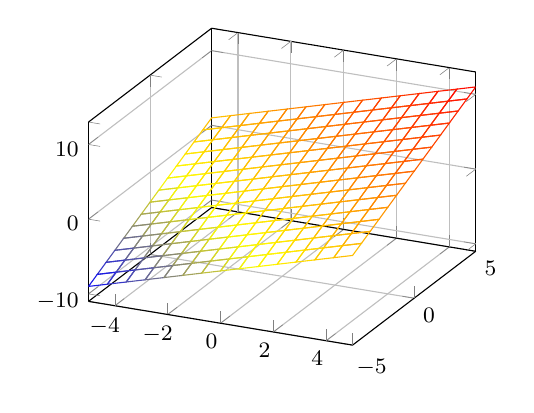
\begin{tikzpicture}
    \begin{axis}[grid=major,small]
      \addplot3 [mesh, samples=15, domain=-5:5] {x+y+1};
    \end{axis}
  \end{tikzpicture}
\end{center}
\end{itemize}
\end{frame}
\begin{frame}[label={sec:org19f761f}]{Application}
\begin{itemize}
\item Feature extraction is important in remote sensing because:
\begin{itemize}
\item It reduces the size of the data,
\item It limits the spatial and spectral redundancy,
\item It permits visualization of the data,
\item It mitigates the \emph{curse of dimensionality}.
\end{itemize}
\item Extraction techniques:
\begin{itemize}
\item Spectral
\begin{itemize}
\item Physically based method,
\item Statistical methods.
\end{itemize}
\item Spatial:
\begin{itemize}
\item Linear filters,
\item Non linear techniques (Mathematical Morphology)
\end{itemize}
\end{itemize}
\end{itemize}
\end{frame}


\section{Physical Indices}
\label{sec:org38aefb3}
\subsection{Introduction}
\label{sec:orga617182}
\begin{frame}[label={sec:org0709c32}]{Spectral indices}
\begin{itemize}
\item Spectral indices are a linear/non-linear combination of two (or more) spectral bands.
\item They provides information as a \emph{single number} about:
\begin{itemize}
\item Plant structure,
\item Biochemistry,
\item Humidity,
\item Stress.
\end{itemize}
\item Four main types \cite{hrsv:2011}:
\begin{center}
\begin{tabular}{ll}
\toprule
Name & Formulae\\
\midrule
Difference vegetation index & \(R_{\lambda_1} - R_{\lambda_2}\)\\
Ration vegetation index & \(\dfrac{R_{\lambda_1}}{R_{\lambda_2}}\)\\
Normalized difference vegetation index & \(\dfrac{R_{\lambda_1} - R_{\lambda_2}}{R_{\lambda_1} + R_{\lambda_2}}\)\\
Soil-adjusted vegetation index & \((1+L)\times\dfrac{R_{\lambda_1} - R_{\lambda_2}}{R_{\lambda_1} - R_{\lambda_2}+L}\)\\
\bottomrule
\end{tabular}
\end{center}
\item \emph{The three last indexes are invariant to  a multiplicative factor}
\end{itemize}
\end{frame}

\begin{frame}[label={sec:org6369441}]{Conventional Indices}
Index database : \url{http://www.indexdatabase.de/}

\begin{center}
\small
\begin{tabular}{ll}
\toprule
Name & Formulae  (\(\lambda\) nm)\\
\midrule
Normalized Difference Vnegetation index & \(\dfrac{R_{\lambda_{800}} - R_{\lambda_{670}}}{R_{\lambda_{800}} + R_{\lambda_{670}}}\)\\
Modified Soil-Adjusted Vegetation Index & \(\dfrac{1}{2}\left[2R_{\lambda_{800}}+1 - \sqrt{(2R_{\lambda_{800}}+1)^2-8(R_{\lambda_{800}}-R_{\lambda_{670}})}\right]\)\\
Modified Chlorophyll Absorption Ratio Index & \(\left[(R_{\lambda_{700}}-R_{\lambda_{670}})-0.2(R_{\lambda_{700}}-R_{\lambda_{550}})\right]\times\dfrac{R_{\lambda_{700}}}{R_{\lambda_{670}}}\)\\
\midrule
Normalized Difference Water Index & \(\dfrac{R_{\lambda_{858}} - R_{\lambda_{1240}}}{R_{\lambda_{858}} + R_{\lambda_{1240}}}\)\\
Datt Reflectance Index & \(\dfrac{R_{\lambda_{816}} - R_{\lambda_{2218}}}{R_{\lambda_{816}} + R_{\lambda_{2218}}}\)\\
\midrule
Normalized Difference Redness Index & \(\dfrac{R_{\lambda_{540}} - R_{\lambda_{700}}}{R_{\lambda_{540}} + R_{\lambda_{700}}}\)\\
Soil Brightness Index & \(0.406R_{\lambda{550}}+0.600R_{\lambda{650}}+0.645R_{\lambda{750}}+0.243R_{\lambda{950}}\)\\
\bottomrule
\end{tabular}
\end{center}
\end{frame}

\subsection{Vegetation Indices}
\label{sec:orgef9baf6}
\begin{frame}[label={sec:orga5f0f7c}]{Normalized difference vegetation index}
$$\text{NDVI}=\dfrac{R_{\lambda_{800}} - R_{\lambda_{670}}}{R_{\lambda_{800}} + R_{\lambda_{670}}}$$
\begin{itemize}
\item \(-1\leq \text{NVDI} \leq 1\)
\item \(\text{NDVI}\leq 0\): surfaces other thatn plant cover
\item \(\text{NDVI}\approx 0\): bare soil
\item \(\text{NDVI}\geq 0.1\): vegetation cover (higher values correspond to more dense covers)
\end{itemize}

\begin{center}
\begin{tikzpicture}
\begin{axis}[xmin=0.4,xmax=1,ymin=0,ymax=1,grid,xlabel=$\lambda~({\mu}m)$,ylabel=Reflectance,width=0.6\linewidth,height=0.3\linewidth,cycle list name=color list]
  \addplot+[mark=none,thick,smooth] file {../Introduction/figures/oak.txt};
  \pgfplotstableread{../Introduction/figures/grass.txt}\loadedtable
  \addplot+[mark=none,smooth,thick] table[x=wave,y=grass] from \loadedtable;
  \addplot+[mark=none,smooth,thick] table[x=wave,y=drygrass] from \loadedtable;
  \pgfplotstableread{../Introduction/figures/talc.txt}\loadtable
  \addplot+[mark=none,smooth,thick] table[x=wave,y=talc] from \loadtable;
  \legend{0.81,0.90, 0.05, -0.03}
\end{axis}
\end{tikzpicture}
\end{center}
\end{frame}

\begin{frame}[label={sec:orge334623}]{}
\end{frame}
\subsection{Case study}
\label{sec:orge0f6c42}
\section{Statistical Feature Extraction}
\label{sec:org8004899}

\subsection{Unsupervised}
\label{sec:org5c9c318}

\subsection{Supervised}
\label{sec:org6ed1534}

\section{Spatial feature extaction}
\label{sec:org5010dc7}

\subsection{Linear filters}
\label{sec:org3a79d19}

\subsection{Mathematical morphology}
\label{sec:org0cb2693}
\end{document}